%% Benjamin Williams <b.williams@staffs.ac.uk>
%% Get in touch if you have any questions or problems!
%% Generic Computer Science Thesis Template
%% (previously lincolncsthesis)

%% @version     1.0.8
%% @lastchanged 04/07/2025

% The document class -- add [harvard] if you want
% harvard-style referencing. You can also add the option
% [sfdefault] if you want the font to be sans-serif. You can 
% also add [centerPageNums] to centre footer page numbers.
\documentclass[]{csthesis}

% Custom packages that you need to include
\input{preamble/packages.tex}

% Your thesis details -- edit the file at the path below
% so it shows your name, title, etc. 
\input{preamble/thesis-details.tex}

% Set up the bib files which are gonna be used
% throughout this document
\input{preamble/bib-setup.tex}



\begin{document}

% start of document
% --------------------------

% Make the title. You can pass an option to this
% to render the title differently, like so:
%\maketitle[logo-first]
\maketitle

% And so begins the thesis! First include pages
% before the acknowledgements
\input{chapters/blank-pages.tex}

% Acknowledgements
\input{chapters/acknowledgements.tex}

% The abstract of the thesis
\input{chapters/abstract.tex}

% Print out the table of tables and table of figures and
% tell the template we're about to start the body of the
% thesis.
\thesisTables
\thesisBodyStart


% start of thesis body
% ---------------------------

% Include introduction
\chapter{Introduction}
\section{Background and Motivation}
It is worth noting that this document was an \textbf{unofficial} thesis template for the University of Lincoln School of Computer Science. Since then, it has changed to encompass a broad range of theses. A decent template was needed for my thesis, so I made this. Then, other people liked it and decided to use it. Along the way, I've added in small features which people have suggested. If you have any suggestions or issues, please contact me -- my email can be found at the top of \texttt{main.tex}! The following subsection in this document demonstrates some capabilities of the template (such as setting your thesis title, and so forth). I have not covered how to use \LaTeX, as this assumes a working knowledge of the language.

If you are from another institution, then I want to thank you for your interest in my template! I've tried to make the template as lightweight as possible so you can modify it to your needs. You can easily swap out the logo (by changing logo.pdf or using \textbackslash thesisLogoPath) and customise the title page contents using the commands listed on the next page. The template is also lightweight enough to enable you to change the typeface of the entire document. Again, if you have any questions please drop me an email as I love hearing your stories!

\section{Problem Statement and Goals}
The \texttt{csthesis} template has a number of definable variables which can be redefined to change the format of the thesis. These are listed below (on the next page).

\vspace{1cm}
\begin{longtable}{l|p{1.3in}|l}
    \bfseries Command & \bfseries Description & \bfseries Example  \\ \hline
    \textbackslash thesisLogoPath & Sets the path to the logo for the title. & \textbackslash thesisLogoPath\{img/your-logo-here.jpg\}  \\
    \textbackslash thesisSubmissionDate & Manually sets the submission date of the thesis, for the title page. & \textbackslash thesisSubmissionDate\{July, 2019\}  \\
    \textbackslash thesisDegree & Sets the name of the degree for this thesis. & \textbackslash thesisDegree\{Doctor of Philosophy\}  \\
    \textbackslash thesisProgramme & Sets the name of your degree programme/subject. & \textbackslash thesisProgramme\{Biology\}  \\
    \textbackslash thesisSupervisor & Sets the name of your supervisor (optional). & \textbackslash thesisSupervisor\{Dr. Mantis Toboggan\}  \\
    \textbackslash thesisSecondSupervisor & Sets the name of your second supervisor (optional). & \textbackslash thesisSecondSupervisor\{Dr. Mantis Toboggan\}  \\
    \textbackslash thesisThirdSupervisor & Sets the name of your third supervisor (optional). & \textbackslash thesisThirdSupervisor\{Dr. Mantis Toboggan\}  \\
%    \textbackslash thesisStudentNumber & Sets your student number (optional). & \textbackslash thesisStudentNumber\{ABC1234567\}  \\
    %\textbackslash thesisModuleCode & Sets your module code for dissertation theses (optional). & \textbackslash thesisModuleCode\{CMP3000M\}  \\
    \textbackslash thesisSchool & Sets the name of your school. & \textbackslash thesisSchool\{School of Chemistry\}  \\
    \textbackslash thesisCollege & Sets the name of your college. & \textbackslash thesisCollege\{College of Science\}  \\
    \textbackslash thesisUniversity & Sets the name of your university. & \textbackslash thesisUniversity\{University of Lincoln\}  \\
\end{longtable}

In addition, \texttt{\textbackslash thesisSubmissionText\{text\}} overrides the submission statement text, so you can type whatever you'd like onto the front page. This is optional, though. For example, if you wish to erase it entirely, you can use \texttt{\textbackslash thesisSubmissionText\{\}}. Example usage can be found in \texttt{preamble/thesis-details.tex}.




\section{Referencing}
If you have included \texttt{[harvard]} in the document class command, then you will be able to cite things inline with parentheses. You can do this by using \texttt{\textbackslash citep\{citekey\}}. It will print out something like this \citep{aad2012observation}. Or alternatively, you can use \texttt{\textbackslash cite\{citekey\}} to cite things like this \cite{chatrchyan2012observation}. If you wish to use numeric style citing, just remove the \texttt{[harvard]} option from the \texttt{\textbackslash documentclass} command.

This template uses Bib\LaTeX~for referencing, with a Biber backend. This is primarily due to the extensive features Bib\LaTeX~provides, along with the option of glossaries. If you want to customise the referencing style, you can either modify the template slightly to use different options, or use \texttt{\textbackslash usepackage} again to reimport it. There's probably some commands to change its options after its been imported too.

If you wish to use numeric style citations instead, please remove the \texttt{[harvard]} option from your \texttt{\textbackslash documentclass} command. 

\subsection{Ludography}
This thesis template also contains an optional ludography. To use this, just put references into your bib file as usual with the game's details. Then, make sure \texttt{keywords} is set to \texttt{\{game\}}. This is what is used to determine which references are games, and which are actual papers. For a more elaborate example, see \texttt{bib/ludography.bib}.

Also, make sure that the \texttt{title} key is actually the author of the game, and the \texttt{author} is the title of the game. The reason this is swapped around is because Bib\LaTeX~likes to print references out with the author first.

Then, just add \texttt{\textbackslash printLudography} with an optional title argument to print out all citations like \texttt{\textbackslash printLudography} or \texttt{\textbackslash printLudography[Games]}.

You can also use the \texttt{ludography} environment if you wish to print out some text before the list of games is printed. An example of this can be seen in \texttt{main.tex}.

To cite games, you can \texttt{\textbackslash cite} it like any other reference. However, if you want it to display the title instead of the standard referencing style, you can use \texttt{\textbackslash citeGame} instead.

Here is an example of a cited game with a normal reference style: ~\cite{spaceinvaders}. Ugh, pretty ugly. Instead, here the two are  cited in the next sentence as games with \texttt{\textbackslash citeGame}. Both \citeGame{spaceinvaders} and \citeGame{breakout} were games made by Atari. Much better!



% Related work 
\chapter{Related Work}
\section{Problem Statement and Goals}

% Method
\chapter{Method}
\section{Requirements)}
\section{Model and Dataset Selection}
\section{Concept and design}
\subsection{GUI Application}
\subsection{Validation and Benchmarking Pipeline}
\subsection{Performance Evaluation (CPU vs GPU)}
\subsection{Custom Dataset Integration}







Here is a sentence, and you can see a nice picture in Figure \ref{fig:duck}. You can also use the \kbd{autoref} command to do this automatically, like this:~\autoref{fig:duck}.

\begin{figure}[h]
    \centering
    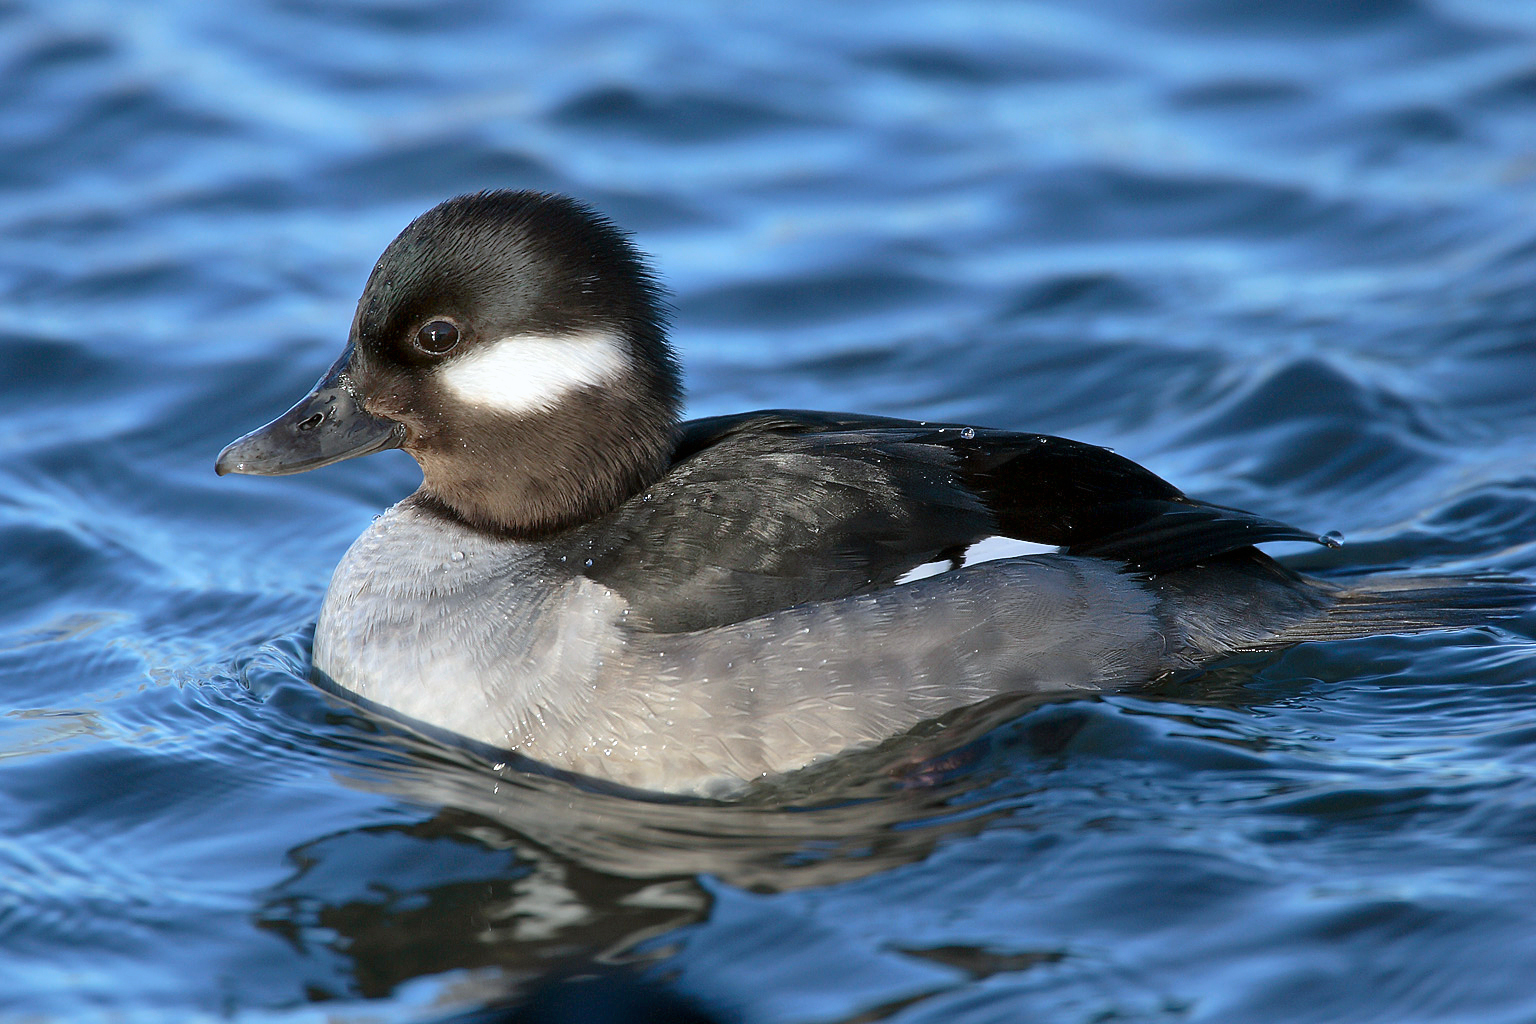
\includegraphics[width=\linewidth]{figures/duck.jpg}
    \caption{A picture of a duck.}
    \label{fig:duck}
\end{figure}

Also, a table can be found in Table \ref{tbl:example-table}. You should use a \LaTeX~table generator like \url{https://www.tablesgenerator.com/} if you want to make your life easier.

\begin{table}[h]
    \caption{Here is a table. The caption goes above like this.}
    \centering
    \begin{tabular}{l|l|c}
        First name & Last name & Age \\
        \hline\hline
        Bob & Bobbington & 24 \\
        Benth & Wavies & 49 \\
        Joe & Bloggs & 37 \\
        Billy & Bob & 10 \\

    \end{tabular}
    \label{tbl:example-table}
\end{table}

% Conclusions
\chapter{Conclusions}
\input{chapters/conclusions.tex}


% end of thesis body
% --------------------------

% Print out the references
\printReferences

% Print out the ludography (optional)
\printLudography

% If you want to put some text before the list of games,
% then you can use the following code:
%\begin{ludography}[Ludography / Optional Title]
    %Here are some games.
%\end{ludography}


\end{document}
